\documentclass[12pt,a4paper]{article}
%\usepackage{epsf,epic,eepic,eepicemu}
%\documentstyle[epsf,epic,eepic,eepicemu]{article}

\usepackage[pdftex]{graphicx}
\usepackage[utf8]{inputenc} %kodovani znaku v textovem souboru
%\usepackage[T1]{fontenc} %kodovani znaku na vystupu
\usepackage[czech]{babel} %prizpusobeni jazyku, napr. deleni slov
%\usepackage{a4wide}

\begin{document}
\title{Semestrální projekt MI-PPR.2 2014/2015\\
Paralelní algoritmus pro řešení problému \\
\vspace{10px}}
\author{Karel Fiala \\ Michal Kučera \\
\vspace{10px} \\
\small České vysoké učení technické v Praze\\
\small Fakulta informačních technologií\\
\small Thákurova 9, 160 00 Praha 6\\
\small Česká republika \\
\vspace{10px} \\
}
\date{\today}
\maketitle

%\oddsidemargin=-5mm \evensidemargin=-5mm \marginparwidth=.08in
%\marginparsep=.01in \marginparpush=5pt \topmargin=-15mm
%\headheight=12pt \headsep=25pt \footheight=12pt \footskip=30pt
%\textheight=25cm \textwidth=17cm \columnsep=2mm \columnseprule=1pt
%\parindent=15pt\parskip=2pt

%Zpráva má obsahovat minimálně následující body:

%Definici problému
%Popis sekvenčního algoritmu a jeho implementace
%Popis paralelního algoritmu a jeho implementace, včetně odůvodnění volby algoritmu pro hledání dárce a metody dělení zásobníku
%Tabulkově a případně graficky zpracované naměřené hodnoty časové složitosti měřených instancí běhu programu s popisem instancí dat
%Analýza a hodnocení vlastností paralelního programu, zvláště jeho efektivnosti a škálovatelnosti, vzniku superlineárního zrychlování a srovnání komunikační režie stejných instancí nad Ethernetem a Infinibandem.
%Závěr
%Literatura

\clearpage
\tableofcontents
\clearpage

\section{Definice problému a popis sekvenčního algoritmu}

%Popište problém, který váš program řeší. Jako výchozí použijte text
%zadání, který rozšiřte o přesné vymezení všech odchylek, které jste
%vůči zadání během implementace provedli (např.  úpravy heuristické
%funkce, organizace zásobníku, apod.). Zmiňte i případně i takové
%prvky algoritmu, které v zadání nebyly specifikovány, ale které se
%ukázaly jako důležité.  Dále popište vstupy a výstupy algoritmu
%(formát vstupních a výstupních dat). Uveďte tabulku nameřených časů
%sekvenčního algoritmu pro různě velká data.

\subsection{Úloha PEK: Permutace číselných koleček}

\subsubsection{Vstupní data}

n = délka rovnostranného trojúhelníka, n>=5 
q = přirozené číslo, n na 2>q 
X0 = počáteční konfigurace zkonstruovaná zpětným provedením q náhodných tahu z cílové konfigurace. Platí q>=d(X0). 

\subsubsection{Pravidla a cíl hry}

Herní deska má tvar rovnostranného trojúhelníka o délce strany n, kde v i-tem řádku je i políček, ležících na průsečících úseček, rovnoběžných se stranami trojúhelníka. V těchto políčkách jsou podle určité permutace rozmístěna kolečka s čísly 1,…,M-1, kde M=n(n+1)/2. Jedno políčko zůstává volné, viz příklad na obrázku vlevo.

\begin{figure}[ht]
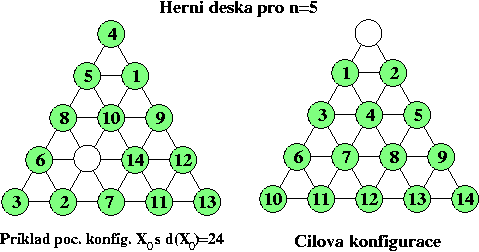
\includegraphics[width=\textwidth]{pek.png}
\caption{Hrací plocha}
\label{pek}
\end{figure}

Tomuto rozmístění koleček budeme říkat počáteční konfigurace X0. Jeden tah je přesun kolečka na sousední volné políčko ve směru některé úsečky. Cílem hry je použitím minimálního počtu tahů převést počáteční konfiguraci X0 do cílové konfigurace C, ve které jsou kolečka seřazena vzestupně po řádcích tak, že políčko na horním vrcholu trojúhelníkové desky je volné, viz obrázek vpravo. Úloha má vždy řešení.

\subsubsection{Definice}

Je-li X konfigurace rozmístění všech koleček na herní desce, pak

t(X) je počet doposud provedených tahů, kterými jsme převedli počáteční konfiguraci X0 do konfigurace X.
d(X) je spodní mez počtu tahů, kterými se lze dostat z konfigurace X do cílové konfigurace C. Tato spodní mez je rovna součtu vzdáleností koleček od jejich cílových políček. Vzdálenost 2 políček v této síti se počítá takto: Jsou-li obě políčka na úsečce rovnoběžné se stranou trojúhelníka, pak je vzdálenost rovna jejich lineární vzdálenosti po této úsečce. V opačném případě tvoří políčka vrcholy kosodélníka a vzdálenost se rovná součtu délek jeho dvou stran. Spodní mez počtu tahů nejlepšího možného řešení je tedy d(X0).
Generování počátečního stavu:

X0 vygenerujeme nejprve q náhodně provedenými zpětnými tahy z cílové konfigurace C.

\subsubsection{Výstup algoritmu}

Výpis nejkratší posloupnosti tahů vedoucí z počáteční konfigurace do cílové konfigurace.

\subsubsection{Sekvenční algoritmus}

Sekvenční algoritmus je typu BB-DFS s neomezenou hloubkou stromu konfiguraci. Přípustný stav je cesta z počáteční do cílové konfigurace C. Cena, která se minimalizuje, je počet tahů takové cesty.

Horní mez počtu tahů je q.

Dolní mez je d(X0).

\subsubsection{Paralelní algoritmus}

Paralelní algoritmus je typu L-PBB-DFS-D.



\section{Popis paralelního algoritmu a jeho implementace v MPI}

Popište paralelní algoritmus, opět vyjděte ze zadání a přesně
vymezte odchylky, zvláště u algoritmu pro vyvažování zátěže, hledání
dárce, ci ukončení výpočtu.  Popište a vysvětlete strukturu
celkového paralelního algoritmu na úrovni procesů v MPI a strukturu
kódu jednotlivých procesů. Např. jak je naimplementována smyčka pro
činnost procesů v aktivním stavu i v stavu nečinnosti. Jaké jste
zvolili konstanty a parametry pro škálování algoritmu. Struktura a
sémantika příkazové řádky pro spouštění programu.

\section{Naměřené výsledky a vyhodnocení}

\begin{figure}[ht]
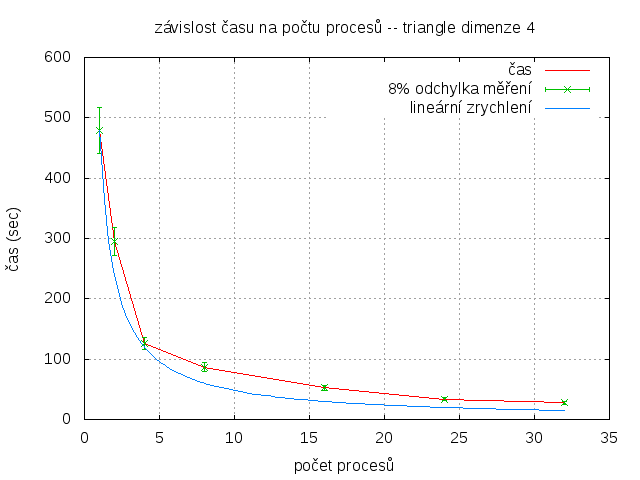
\includegraphics[width=\textwidth]{data4.png}
\caption{Měření pro trojúhelník dimenze 4}
\label{data4}
\end{figure}

\begin{figure}[ht]
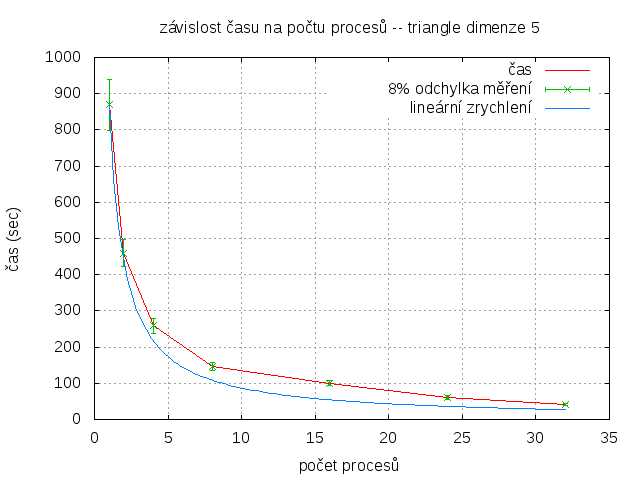
\includegraphics[width=\textwidth]{data5.png}
\caption{Měření pro trojúhelník dimenze 5}
\label{data5}
\end{figure}

\begin{figure}[ht]
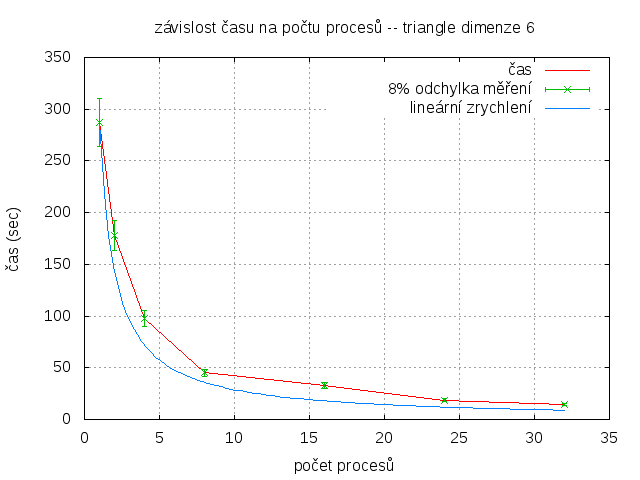
\includegraphics[width=\textwidth]{data6.png}
\caption{Měření pro trojúhelník dimenze 6}
\label{data6}
\end{figure}

\begin{enumerate}
\item Zvolte tři instance problému s takovou velikostí vstupních dat, pro které má
sekvenční algoritmus časovou složitost kolem 5, 10 a 15 minut. Pro
meření čas potřebný na čtení dat z disku a uložení na disk
neuvažujte a zakomentujte ladící tisky, logy, zprávy a výstupy.
\item Měřte paralelní čas při použití $i=2,\cdot,32$ procesorů na sítích Ethernet a InfiniBand.
%\item Pri mereni kazde instance problemu na dany pocet procesoru spoctete pro vas algoritmus dynamicke delby prace celkovy pocet odeslanych zadosti o praci, prumer na 1 procesor a jejich uspesnost.
%\item Mereni pro dany pocet procesoru a instanci problemu provedte 3x a pouzijte prumerne hodnoty.
\item Z naměřených dat sestavte grafy zrychlení $S(n,p)$. Zjistěte, zda a za jakych podmínek
došlo k superlineárnímu zrychlení a pokuste se je zdůvodnit.
\item Vyhodnoďte komunikační složitost dynamického vyvažování zátěže a posuďte
vhodnost vámi implementovaného algoritmu pro hledání dárce a dělení
zásobníku pri řešení vašeho problému. Posuďte efektivnost a
škálovatelnost algoritmu. Popište nedostatky vaší implementace a
navrhněte zlepšení.
\item Empiricky stanovte
granularitu vaší implementace, tj., stupeň paralelismu pro danou
velikost řešeného problému. Stanovte kritéria pro stanovení mezí, za
kterými již není učinné rozkládat výpočet na menší procesy, protože
by komunikační náklady prevážily urychlení paralelním výpočtem.

\end{enumerate}

\section{Závěr}

Celkové zhodnocení semestrální práce a zkušenosti získaných během
semestru.

\section{Literatura}

\appendix


\end{document}
